\chapter{Instrumentation de la source secondaire}\label{chap:InstrumHP}
\section{Objectif}
Le déphasage des sources est un critère primordial pour l'obtention des meilleurs performances possibles avec cette machine. Au démarrage de la thèse, seule la source acoustique principale est munie d'un accéléromètre, et la phase de chaque source n'est réglée que sur le générateur basse fréquence utilisé. La source acoustique secondaire est instrumentée afin de connaître avec précision le déplacement de son piston, sans pour autant perturber le système global en modifiant ses paramètres électroacoustiques après l'ajout d'un accéléromètre.

\section{Choix du capteur}
L'accéleromètre à fixer sur la source acoustique secondaire doit être le plus petit possible pour modifier le moins possible ses paramètres de Thiele et Small. Le modèle retenu est l'accéléromètre 352C23 du fabricant PCB Piezotronics. Sa masse est de \echaf{masse ?}. 

Il est souhaité un grand déplacement des sources acoustiques, ainsi qu'une puissance acoustiqe la plus élevée possible. La fréquence de travail doit donc être inférieure ou égale à la fréquence de résonance de chacune des sources. Dans le cas de la source secondaire \echaf{on est en dessous parce que la pression est proportionnelle au déplacement car volume fermé, donc même si ajout de masse on reste inférieur à fc du hp}


\section{Montage}
L'installation de l'accéléromètre est difficile : il n'est pas possible de fixer l'accéléromètre sur la face arrière de la source acoustique, et la distance entre la face avant et l'échangeur ambiant n'est que de \echaf{\qty{2}{\milli\meter}}. De plus, la traversée qui connecte la source acoustique à l'extérieur de la machine se trouve du côté de la face arrière, complètement séparée de la face avant. La solution retenue est de réaliser un perçage au centre du piston pour y faire passer le câble du capteur, puis de le reboucher avec de la colle. La source secondaire instrumentée est présentée sur la figure~\ref{fig:HPPeerless_WithAcc}.

\begin{figure}[!ht]
    \centering
    \external{fig_HPPeerless_WithAcc}
    %\externalremake
    \tikz{\draw(0,0) node{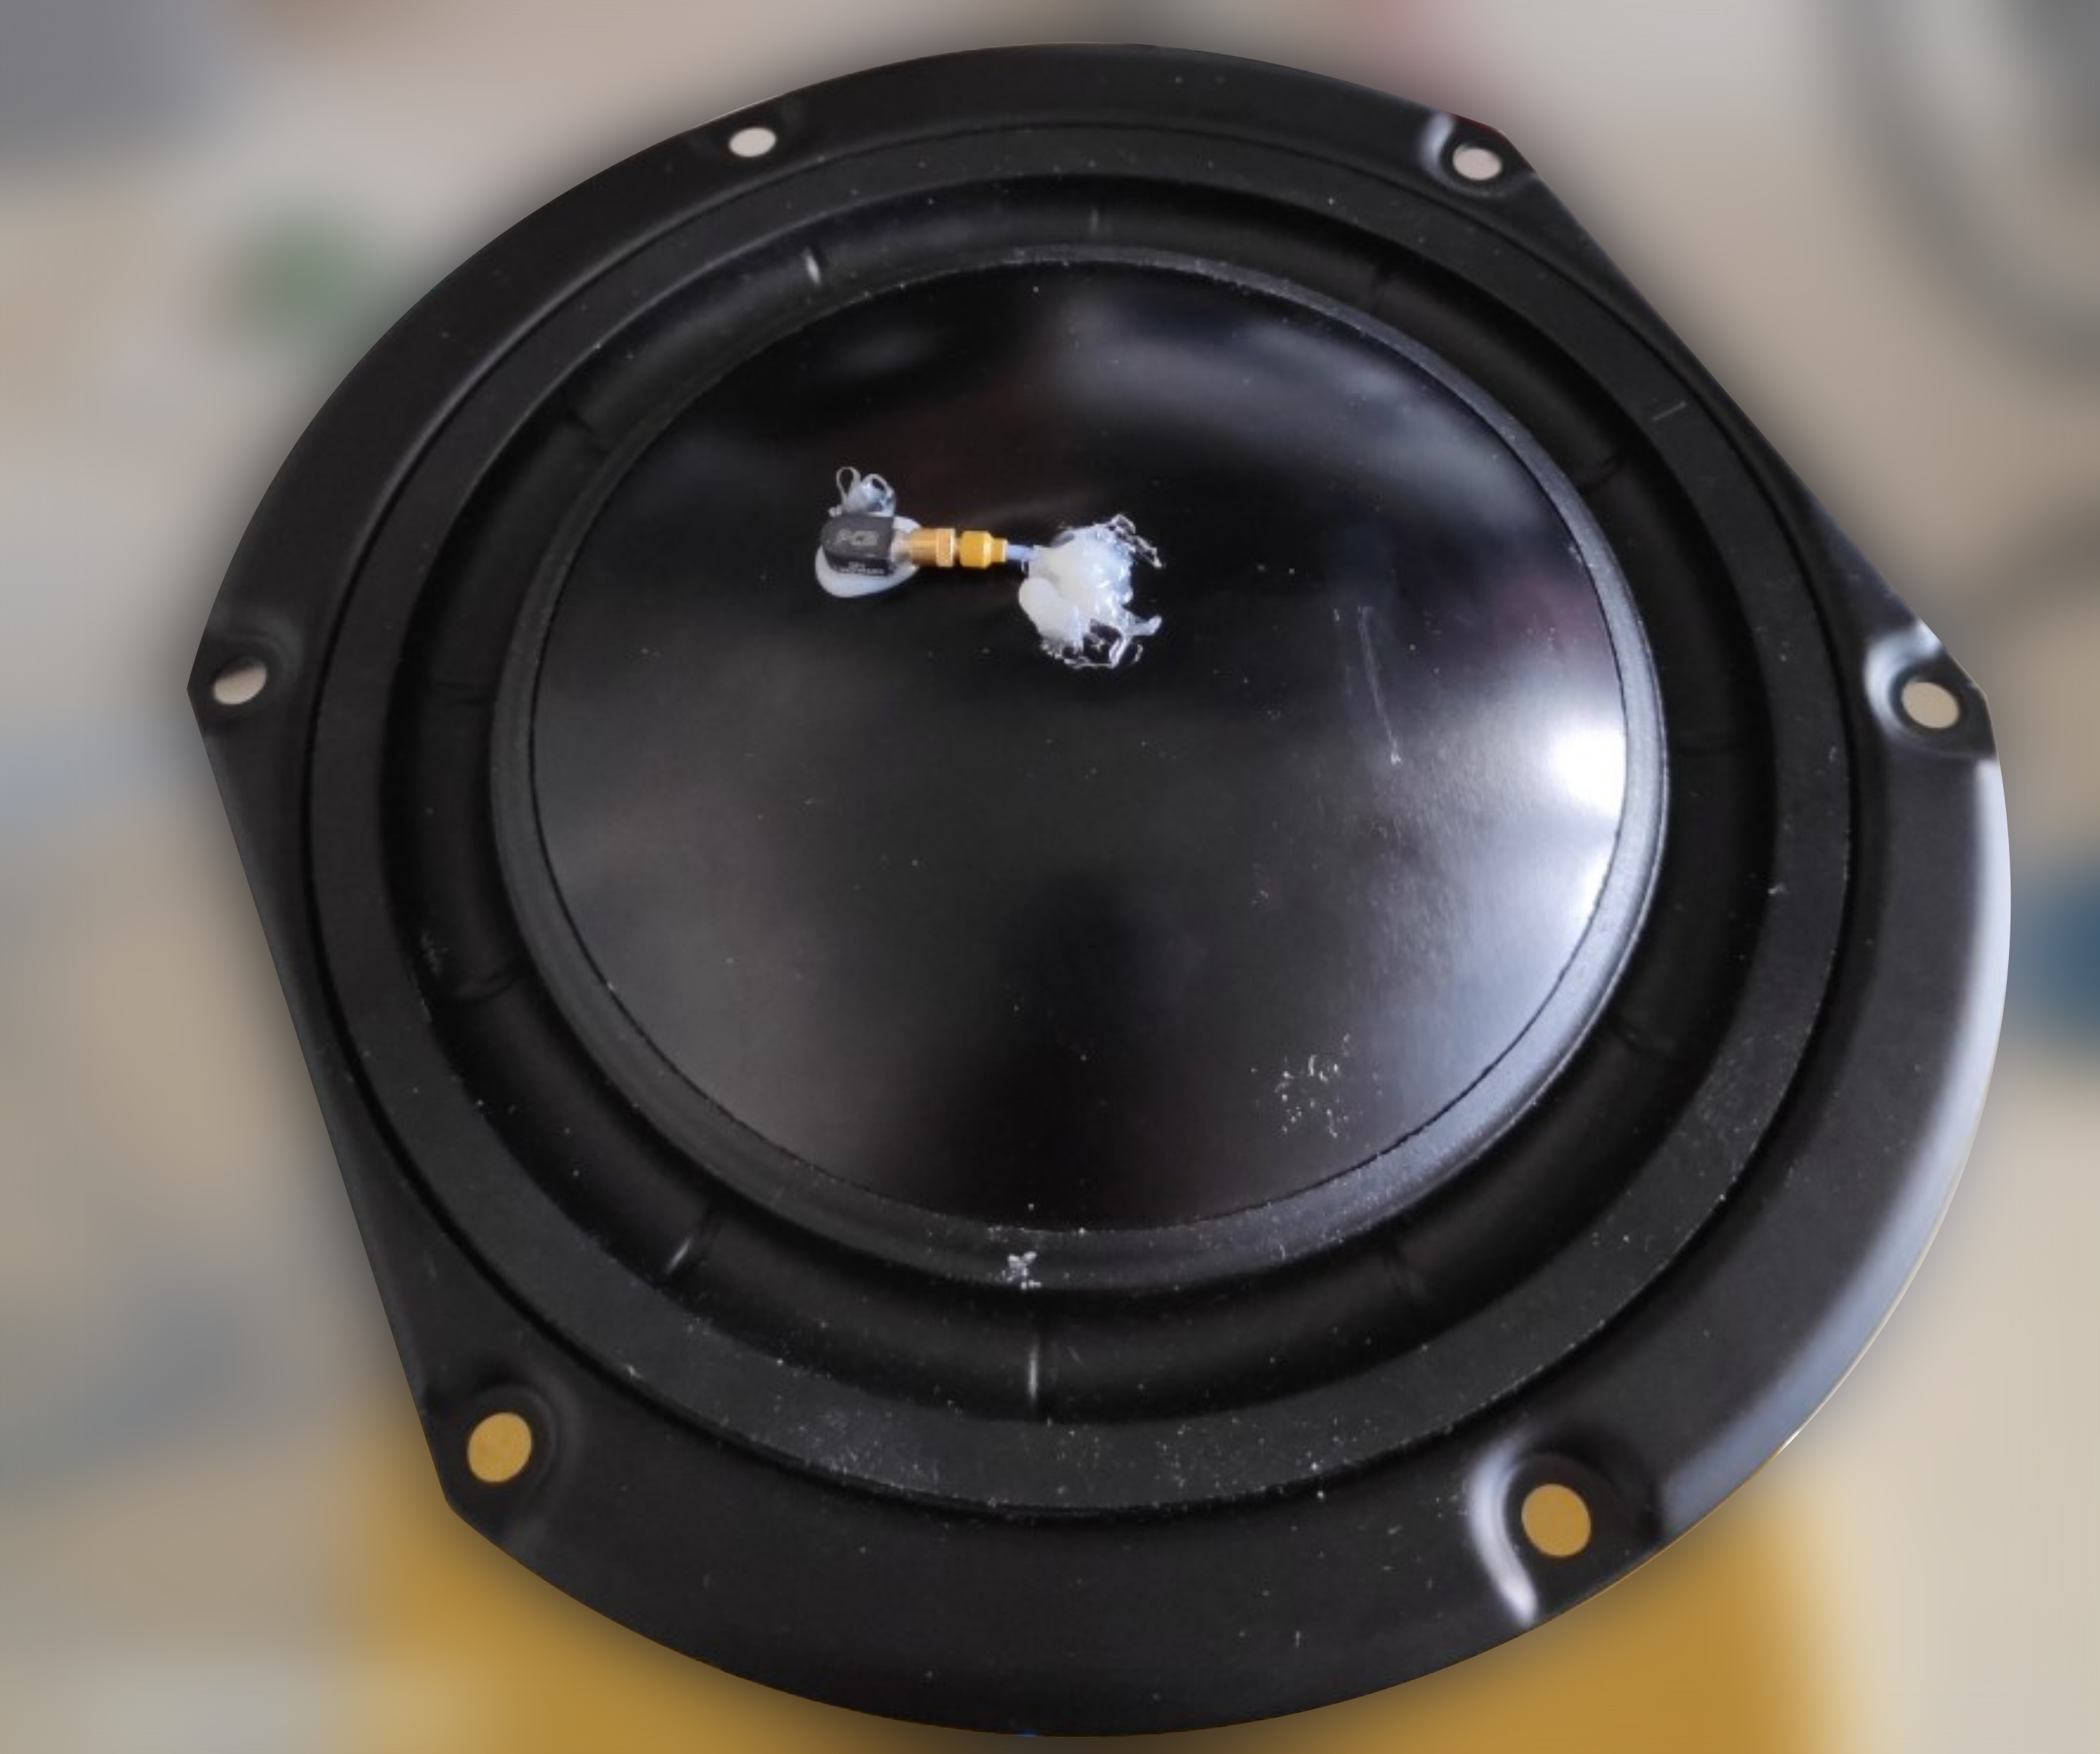
\includegraphics[width=.7\textwidth]{../fig/fig_InstrumentationHP/HPPeerless_WithAcc.png}};}
    \caption{Source acoustique secondaire avec l'accéléromètre collé sur sa membrane.}
    \label{fig:HPPeerless_WithAcc}
\end{figure}

\section{Vérification}
\subsection{Banc de mesures}

\subsection{Résultats}